\documentclass[sigconf,nonacm,anonymous]{acmart}

\usepackage{booktabs}
\usepackage{multirow}
\usepackage{array}
\usepackage{xspace}
\usepackage{algorithm}
\usepackage{algpseudocode}
\usepackage{tikz}
\usetikzlibrary{positioning,arrows.meta,calc,fit,patterns,decorations.pathreplacing}

\settopmatter{printfolios=true}

% ---- names used consistently throughout -----------------------------------
\newcommand{\cc}{\textsc{CC}\xspace}
\newcommand{\cctwo}{\textsc{CC-2PL}\xspace}
\newcommand{\ccs}{\textsc{CC-$\sigma$}\xspace}
\newcommand{\mtpo}{\textsc{MTPO}\xspace}
\newcommand{\seal}{\mathsf{seal}}
\newcommand{\cell}[1]{\texttt{#1}}
\newcommand{\eg}{e.g.,\xspace}
\newcommand{\ie}{i.e.,\xspace}

\newtheorem{theorem}{Theorem}
\newtheorem{lemma}{Lemma}
\newtheorem{corollary}{Corollary}
\newtheorem{proposition}{Proposition}
\newtheorem{definition}{Definition}

% colours shared by the TikZ figures and the plots
\definecolor{ccblue}{HTML}{2A78D6}
\definecolor{ccorange}{HTML}{EB6834}
\definecolor{ccaqua}{HTML}{1BAF7A}
\definecolor{ccmuted}{HTML}{52514E}
\definecolor{ccgrid}{HTML}{D9D8D3}

\begin{document}

\title{Certified Chopping for Agent Tool Workflows: Admitting Plan Revisions over Committed Effects}

\author{Anonymous Author(s)}
\affiliation{\institution{Anonymous Institution}\country{}}

\begin{abstract}
Concurrent AI agents read and write shared application state through tools,
and they interleave badly. Wrapping each tool call in a transaction does not
make an agent's intent atomic; holding a transaction across an entire
reason-and-act workflow serializes long intervals of private reasoning; and
repairing conflicts after the fact makes correctness depend on the judgement
of the model. Transaction chopping is the classical answer to this tension,
but it assumes that transaction programs are fixed before execution. Agents
are not fixed: they revise their plans after observing tool results, by which
time earlier pieces have committed and their effects are visible.

We study the resulting problem, \emph{prefix-aware recertification}: deciding
whether a mid-flight plan revision can be admitted when the past can no longer
be rechopped. We give a complete characterization. A revision is admissible
under future-only repair if and only if \emph{sealing} every workflow's
uncommitted remainder into one piece yields a plan with no mixed
sibling--conflict cycle. The corollary is an impossibility result: when the
residual cycle passes through a committed piece, no regrouping of the future
helps, and neither does waiting for other workflows to finish. We further show
that admission decisions must be serialized.

We build a runtime that makes the certificate's hypotheses true rather than
assumed---mediated, fail-closed footprint enforcement, range footprints for
predicate reads, and piece-level locking---and we study three locking
disciplines inside a piece, the last of which reuses a launch-time priority
order to make deadlock unreachable. Bounded exhaustive checking against a
brute-force serializability oracle finds no unsound admission. With real
language-model agents on twelve workloads and two models, certified chopping
with priority-ordered locking is anomaly-free in 98\% of trials, is
statistically as fast as a state-of-the-art repair-based protocol
($1.33\times$ versus $1.38\times$ over serial execution on contended
workloads), is significantly faster than whole-workflow locking, and never
deadlocks. When it fails, it leaves shared state clean rather than corrupted.
We also report where the approach does not pay: most mid-flight escalations into
shared state are inadmissible, and on workloads whose read-modify-write
straddles the reasoning gap certification correctly collapses to
whole-workflow locking.
\end{abstract}

\keywords{transaction chopping, concurrency control, LLM agents, tool use,
serializability}

\maketitle

\section{Introduction}
\label{sec:intro}

Two agents are asked to resize the same Kubernetes deployment at the same
time. One doubles the replica count to absorb a load spike; the other adds
three replicas for headroom. Each reads the current count, reasons about what
to do, and writes back a new value. Starting from four replicas, the only
defensible outcomes are $11$ (double, then add) and $14$ (add, then double).
We ran this workload with two concurrent language-model agents and no
coordination. In every one of twenty trials, across two different models, both
agents read~$4$ and the final count was $7$ or $8$: one update was lost.
Neither agent reasoned incorrectly. Each computed the right value from what it
read. The anomaly is a concurrency-control failure, and no amount of prompt
engineering removes it.

\paragraph{Three answers, three costs.}
The database community has seen this problem before, and each classical answer
carries over to agents with a specific cost.

\emph{Make every tool call a transaction.} This is what most agent frameworks
do implicitly. It is fast and wrong: the unit an application wants to be
atomic is the agent's \emph{intent}---read, decide, write---not the individual
call, and the lost update above lives precisely in the gap between calls.

\emph{Make the whole workflow a transaction.} This is correct, but the
workflow includes the agent's reasoning, which is by far its longest part.
Holding locks across model inference serializes exactly the interval one
would most like to overlap. In our measurements, whole-workflow two-phase
locking is barely faster than running the agents one after another
($1.06\times$).

\emph{Let agents run, and repair conflicts afterwards.} Recent systems order
agents by a launch-time priority, apply writes speculatively, and notify an
agent when a premise it read has changed, relying on the agent to repair its
own work~\cite{lyu2026coagent}. This is fast, but it moves the correctness
argument into the model: the protocol is serializable only if a notified agent
correctly decides whether its plan is affected and correctly repairs it. We
measure that assumption directly; it holds in 91\% of notified trials for a
small model and 95\% for a large one, and when it fails on an append-only log
the wrong record cannot be withdrawn.

\paragraph{Chopping, and what breaks it.}
Transaction chopping~\cite{shasha1995chopping} resolves the tension between
the first two answers for classical workloads. A transaction is split into
pieces that execute and commit independently, so that locks are released
between pieces, and a static graph test guarantees that every interleaving of
pieces is equivalent to some serial execution of the original transactions.
For an agent, the natural place to cut is the reasoning gap: commit the read,
think without holding anything, then write.

The classical theorem, however, assumes that the set of transaction programs
is known before execution. An agent violates this assumption in a specific,
consequential way: \emph{it decides what to do next after seeing what it just
read}. A support agent reads an order and only then discovers that the
resolution requires touching a shared gift-card balance. By that point the
read has committed and its result has been returned. The plan that was
certified is no longer the plan being executed.

One can recertify the revised plan, and that is sound. The difficulty is what
to do when recertification fails. Before execution, a failed certification is
always repairable: merge pieces until, in the limit, each workflow is a single
piece. After a prefix has committed, that repair is unavailable, because
merging a committed piece with a future one is not a physical operation. The
question is whether some weaker repair always exists. We show that it does
not, and we characterize exactly when it does.

\paragraph{Contributions.}
\begin{itemize}
\item We formalize \emph{prefix-aware recertification}: admitting a plan
  revision against a batch in which some pieces have already committed and
  only the uncommitted suffix may be regrouped (\S\ref{sec:model},
  \S\ref{sec:theory}).
\item We prove a complete characterization (Theorem~\ref{thm:char}): a
  revision is admissible under future-only repair if and only if sealing
  every workflow's uncommitted remainder into one piece yields an
  SC-cycle-free plan. This reduces admission to a single cheap test and tells
  the runtime when searching finer choppings is pointless.
\item We prove the corresponding impossibility result
  (Corollary~\ref{cor:imp})---waiting for concurrent workflows to finish does
  not rescue an inadmissible revision---and show that admission must be
  serialized (Theorem~\ref{thm:serial}).
\item We build a runtime that enforces the certificate's hypotheses rather
  than trusting them (\S\ref{sec:runtime}): every tool access is mediated and
  checked fail-closed against the footprint of the executing piece, predicate
  reads are ranges so that phantoms are visible to certification, and pieces
  are isolated by locking. We study three locking disciplines inside a piece.
  The third, \ccs, orders lock waits by the same launch-time priority that
  repair-based protocols use for notifications, which makes deadlock
  unreachable while keeping holds short.
\item We check every soundness claim against a brute-force serializability
  oracle (\S\ref{sec:verification}) and evaluate with real language-model
  agents on twelve contended workloads, two models, five baselines and
  three variants of our own, 1{,}682 trials in total (\S\ref{sec:eval}).
\end{itemize}

\paragraph{Summary of results.}
With a small model driving both agents, \ccs is anomaly-free in 98\% of
trials, against 96\% for whole-workflow locking and 93\% for the repair-based
protocol. On the contended workloads it is as fast as the repair-based
protocol ($1.33\times$ versus $1.38\times$ over serial; the difference is
not significant) and significantly faster than whole-workflow locking
($+0.27\times$, faster on eight of eight workloads). Where the structure of
the workload permits a cut, it reaches $2.15\times$ while whole-workflow
locking stays at $0.98\times$. It never deadlocks, and in that run it is the
only protocol whose slowest workload is still faster than serial execution.

We are equally explicit about what does not work. On ten of our twelve
workloads a read-modify-write or scan-then-insert straddles the reasoning gap,
and certification correctly refuses to cut there. Most mid-flight escalations
into shared state are inadmissible: between 4\% and 37\% are admitted in a
controlled study, and 19\% with a large model on live agents. Certified
chopping does not remove the dependence on the agent; it relocates it, from
\emph{repairing a record correctly} to \emph{retrying after a refusal}, and
changes what a failure costs.

We do not claim a new isolation theorem for static choppings, a general ACID
protocol for agents, or the first transactional treatment of agent tool use.
Our contribution is the revision-admission problem and its solution, a runtime
that enforces it, and an evaluation that reports both where the approach wins
and where the right answer is not to chop.

\section{Background and Motivation}
\label{sec:background}

\subsection{Agent tool workflows}

An agent is a loop around a language model. In each round the model receives
the task and everything observed so far, and emits either a \emph{tool call}
or a statement that it is done. A tool call reads or writes shared state: a
deployment, a calendar, a customer record. The result of the call is appended
to the model's context, and the loop continues.

Two properties of this loop matter for concurrency control. First, the
interval between two tool calls is a model inference. It takes seconds, it is
private to the agent, and it touches no shared state. We call it the
\emph{reasoning gap}. Second, the sequence of calls is not known in advance:
which tool the agent calls next depends on what the last call returned.

When several agents work on the same system, their tool calls interleave. The
result is the familiar catalogue of anomalies~\cite{bernstein1987}. Two agents
that both read a value, reason, and write a derived value lose an update. An
agent that scans a collection and then acts on what it saw misses an object
another agent inserted in between, a phantom~\cite{eswaran1976}. An agent that
appends a record derived from a value another agent has since overwritten
leaves a log that no serial execution could have produced.

\subsection{Existing answers}

\paragraph{Whole-workflow isolation.} Treating each agent's entire workflow
as one transaction prevents every anomaly above. Under strict two-phase
locking (2PL) the agent holds each lock from first use until it finishes;
under optimistic concurrency control (OCC)~\cite{kung1981occ} it runs
unlocked and validates at the end. Because the target systems that agents
operate on---a Kubernetes API, a CRM---offer neither private workspaces nor
rollback, writes land in place, and an abort is implemented as a
saga~\cite{garciamolina1987sagas}: each tool registers an inverse, and a
victim's writes are undone by running the inverses. The cost of both policies
is tied to the reasoning gap. 2PL holds locks across it; OCC discards a whole
workflow's worth of inference when validation fails.

\paragraph{Ordered repair.} CoAgent~\cite{lyu2026coagent} takes the opposite
position. Its protocol, \mtpo, assigns every agent a rank $\sigma$ at launch
and aims for the outcome of running the agents serially in $\sigma$ order.
Reads return the value the reader would have seen in that order; writes apply
speculatively in place; and when a lower-ranked agent overwrites something a
higher-ranked agent has read, the higher-ranked agent receives a
\emph{notification} carrying the new value. Notifications flow in one
direction only, from lower $\sigma$ to higher. Nobody blocks and nothing is
undone, which makes \mtpo fast. Its correctness, however, rests on two
assumptions about the model: that an agent completes its task correctly in
isolation (A1), and that a notified agent correctly judges whether its plan is
affected and repairs exactly the affected operations (A3). CoAgent assumes
A3 holds 95\% of the time. We return to both assumptions in
\S\ref{sec:eval:agent}.

\subsection{Transaction chopping}

Transaction chopping~\cite{shasha1995chopping} asks a different question:
which transactions can be cut into smaller ones without anyone being able to
tell? A \emph{chopping} splits each transaction into consecutive
\emph{pieces}. Each piece executes as its own serializable transaction and
commits before the next begins, so locks are held only within a piece.

Whether a chopping is safe is decided by an undirected graph over the pieces,
the \emph{SC graph}. Two pieces of the same transaction are joined by an
\emph{S~edge} (sibling). Two pieces of different transactions that access a
common item, at least one of them writing it, are joined by a \emph{C~edge}
(conflict). The chopping is correct---every execution is equivalent to a
serial execution of the \emph{original} transactions---if the graph has no
simple cycle containing both an S~edge and a C~edge.

\begin{figure}[t]
\centering
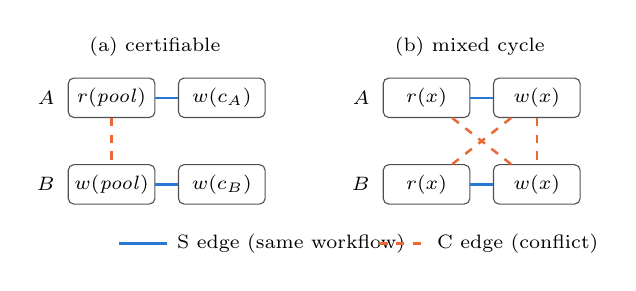
\begin{tikzpicture}[
  piece/.style={draw=ccmuted, rounded corners=2pt, minimum height=5mm,
                minimum width=11mm, font=\scriptsize, inner sep=1.5pt},
  S/.style={ccblue, line width=0.9pt},
  C/.style={ccorange, line width=0.9pt, dashed},
  lab/.style={font=\scriptsize}]
% ---- (a) choppable ------------------------------------------------------
\node[lab] at (1.05,1.75) {(a) certifiable};
\node[lab, anchor=east] at (-0.1,1.1) {$A$};
\node[lab, anchor=east] at (-0.1,0.0) {$B$};
\node[piece] (a1) at (0.5,1.1) {$r(\mathit{pool})$};
\node[piece] (a2) at (1.9,1.1) {$w(c_A)$};
\node[piece] (b1) at (0.5,0.0) {$w(\mathit{pool})$};
\node[piece] (b2) at (1.9,0.0) {$w(c_B)$};
\draw[S] (a1) -- (a2);
\draw[S] (b1) -- (b2);
\draw[C] (a1) -- (b1);
% ---- (b) not choppable --------------------------------------------------
\begin{scope}[xshift=4.0cm]
\node[lab] at (1.05,1.75) {(b) mixed cycle};
\node[lab, anchor=east] at (-0.1,1.1) {$A$};
\node[lab, anchor=east] at (-0.1,0.0) {$B$};
\node[piece] (c1) at (0.5,1.1) {$r(x)$};
\node[piece] (c2) at (1.9,1.1) {$w(x)$};
\node[piece] (d1) at (0.5,0.0) {$r(x)$};
\node[piece] (d2) at (1.9,0.0) {$w(x)$};
\draw[S] (c1) -- (c2);
\draw[S] (d1) -- (d2);
\draw[C] (c1) -- (d2);
\draw[C] (c2) -- (d1);
\draw[C] (c2) -- (d2);
\end{scope}
% ---- legend ---------------------------------------------------------------
\draw[S] (0.6,-0.75) -- (1.2,-0.75) node[right, lab, black] {S edge (same workflow)};
\draw[C] (3.9,-0.75) -- (4.5,-0.75) node[right, lab, black] {C edge (conflict)};
\end{tikzpicture}
\caption{SC graphs for two agent workflows cut at the reasoning gap. (a)~$A$
reads a shared pool and writes a private claim while $B$ updates the pool: the
only conflict joins the two first pieces, no cycle mixes edge types, and the
chopping is safe. (b)~Both agents read and then write the same object: the
cycle $r_A(x)$--$w_A(x)$--$w_B(x)$--$r_A(x)$ mixes an S~edge with C~edges, so
the cut would permit a lost update and each workflow must stay one piece.}
\label{fig:sc}
\end{figure}

Figure~\ref{fig:sc} shows the two cases that matter for agents. When the
shared dependency is short and the work that follows is private, cutting at
the reasoning gap is safe, and the lock on the shared item is released before
the model starts thinking. When a read-modify-write straddles the gap, the
graph has a mixed cycle and the cut must not be made. The repair is always
available before execution: merge pieces. A workflow that is a single piece
has no S~edges, so it cannot be on a mixed cycle.

\subsection{Why agents break the classical setting}

The chopping theorem quantifies over a set of transaction programs that is
fixed before any piece runs. An agent's plan is not fixed. Suppose a workflow
is certified as ``read $x$; then write a private result'', the read commits,
and the agent then decides, on the basis of what it read, that it must also
write a shared item $y$. The certified plan no longer describes the execution.

Two responses are unsound or unavailable. Certifying only the new suffix is
unsound, because the conflicts that close a cycle may run through the pieces
that already committed. Merging the new write into the piece that performed
the read is unavailable, because that piece has committed and released its
locks; other workflows may already have observed its effects or interleaved
with it. What remains is to regroup the \emph{uncommitted} part of the plan,
and the question this paper answers is when that is enough.

\section{Model}
\label{sec:model}

\paragraph{Intents and workflows.}
An \emph{intent} is the unit an application wants to be atomic and isolated:
``roll this deployment back and record that it was done''. An intent is not an
agent. Several agents can cooperate on one intent, and one long-lived agent
can execute many, so the transaction identity follows the delegated work
rather than the process. In this paper each intent is one ordered
\emph{workflow}; internally parallel intents are future work.

\paragraph{Batches, plans and pieces.}
A \emph{batch} $B$ is a finite set of workflow invocations. A workflow $w$ has
a \emph{plan}: an ordered list of \emph{pieces}, each grouping consecutive
steps, where a step is one mediated tool operation. The pieces of one
workflow execute in order, and each commits before the next begins. Distinct
invocations of the same program are distinct workflows; a single
representative instance would miss the interference between two concurrent
invocations of the same program.

\paragraph{Footprints.}
Each piece $p$ carries a declared \emph{footprint} $F(p)$: a set of accesses,
each an exact key or a half-open key range, marked read or write. A range
models a predicate query such as ``every deployment in this namespace''. A
write to a key inside a declared range conflicts with a read of that range,
which is what makes a phantom insertion visible to certification. Two
accesses \emph{conflict} when their items overlap and at least one is a write:
\begin{align*}
\mathit{conflict}(p,q) \iff{} & \exists\, a\in F(p),\, b\in F(q):\\
 & a \text{ and } b \text{ overlap and one is a write.}
\end{align*}

\paragraph{The SC graph.}
The SC graph of a plan is undirected. Its vertices are the pieces of every
workflow in the batch. An S~edge joins every pair of pieces of the same
workflow, so each workflow's pieces form a clique. A C~edge joins conflicting
pieces of different workflows. The forbidden structure is a \emph{mixed simple
cycle}: a simple cycle with at least one S~edge and at least one C~edge. Pure
S~cycles and pure C~cycles are permitted, and a mixed closed walk that repeats
a vertex does not count. A plan with no mixed simple cycle is
\emph{SC-cycle-free}, and we say it \emph{certifies}.

We detect mixed simple cycles by computing the vertex-biconnected components
of the graph and rejecting any component that contains both edge labels. The
test is exact, because any two edges of a biconnected component lie on a
common simple cycle, and it runs in time linear in the size of the graph.

\paragraph{Execution rules.}
A certificate is a statement about a plan; it becomes a statement about an
execution only if the runtime upholds four obligations. These are the
classical execution rules of chopping~\cite{shasha1995chopping}, restated for
a tool runtime:
\begin{enumerate}
\item[\textbf{E1}] Each piece executes serializably with respect to all other
  pieces. Several atomic tool calls grouped under one label are not an atomic
  piece.
\item[\textbf{E2}] The pieces of a workflow execute in program order.
\item[\textbf{E3}] The declared footprint of a piece bounds its actual
  accesses.
\item[\textbf{E4}] A piece aborted by contention is retried until it commits.
\end{enumerate}
E3 is where an agent runtime differs most from a database. A stored procedure
can be analysed; a model-driven agent cannot, and a model-generated
description of what a tool does is not evidence about what it does. The
runtime of \S\ref{sec:runtime} therefore enforces E3 on every call rather than
assuming it.

\paragraph{What a certificate does and does not buy.}
A certificate is a statement about isolation under the declared model.
It is not \emph{atomicity}: independently committed pieces leave a visible
prefix if the process dies, which must be repaired by durable continuation
(\S\ref{sec:runtime}). It is not \emph{consistency}: serializability preserves
an application invariant only if each workflow is individually correct, and a
model that misreads its task produces a serializable wrong answer. It is not
\emph{real-time ordering}: conflict serializability does not imply strict
serializability. And it says nothing about effects outside the modelled
state. A message that has been sent stays sent; a graph cannot create rollback
for a service that does not offer it.

\section{Prefix-Aware Recertification}
\label{sec:theory}

Let a plan $P$ be certified and executing. The \emph{frontier} $\phi$
records, for each workflow $w$, the number $\phi(w)$ of its pieces that have
committed. A workflow $r$ proposes to replace its uncommitted suffix with a
new sequence of pieces, giving a revised plan $P'$. The runtime must decide
whether to admit $P'$ and, if the proposed chopping is too fine, whether it
can be repaired.

\subsection{Soundness of recertification}

\begin{theorem}[Inherited isolation]
\label{thm:inherit}
If $P'$ is SC-cycle-free, its committed prefix is identical to the prefix
actually executed, and the runtime satisfies E1--E4, then the resulting
history is conflict-serializable at workflow granularity.
\end{theorem}

\begin{proof}
The pieces that already ran are, by construction, exactly the prefix pieces of
$P'$ with the footprints they declared, and E3 guarantees that their actual
accesses were inside those footprints. The observed execution is therefore a
legal execution of the chopping $P'$ under the execution rules. The classical
chopping theorem~\cite{shasha1995chopping} applies to $P'$ and yields
equivalence to a serial execution of the workflows of $P'$.
\end{proof}

Theorem~\ref{thm:inherit} is an application of established theory to a revised
plan, not a new isolation theorem. Its force is in the hypothesis:
recertification must cover the \emph{whole} batch, including pieces that have
committed. Certifying only the new suffix discards exactly the conflicts that
close a cycle through the past.

\subsection{What repairs remain after commitment}

Before execution, a rejected chopping is repaired by merging pieces. After
commitment only the uncommitted suffix may be regrouped.

\begin{definition}
$P''$ is a \emph{future-only coarsening} of $P'$ at $\phi$ if the first
$\phi(w)$ pieces of every workflow $w$ are unchanged and the remaining pieces
of $w$ are grouped into contiguous runs. The \emph{sealing}
$\seal(P',\phi)$ is the future-only coarsening that merges each workflow's
entire remainder into a single piece.
\end{definition}

\begin{lemma}[Sealing is coarsest]
\label{lem:coarsest}
Every future-only coarsening of $P'$ at $\phi$ is a refinement of
$\seal(P',\phi)$.
\end{lemma}

\begin{proof}
Both agree on the committed prefix. Sealing places each workflow's whole
remainder in one piece; any other future-only coarsening partitions that same
remainder into contiguous runs, which is a refinement of the single piece.
\end{proof}

\begin{lemma}[Cycles persist under refinement]
\label{lem:persist}
If a chopping contains a mixed simple cycle, so does every refinement of it.
\end{lemma}

This is the classical non-removability property of
chopping~\cite{shasha1995chopping}: splitting a piece adds S~edges among the
parts and distributes the piece's C~edges among them, so a mixed cycle through
the original piece survives as a mixed cycle through its parts.

\begin{theorem}[Admissibility characterization]
\label{thm:char}
A revision is admissible under future-only coarsening if and only if
$\seal(P',\phi)$ is SC-cycle-free.
\end{theorem}

\begin{proof}
($\Leftarrow$) If the sealing is SC-cycle-free, it is itself a certified
future-only coarsening, so the revision is admissible.
($\Rightarrow$) Suppose the sealing contains a mixed simple cycle. By
Lemma~\ref{lem:coarsest} every future-only coarsening is a refinement of the
sealing, and by Lemma~\ref{lem:persist} every such refinement contains a mixed
simple cycle. Hence no future-only coarsening certifies.
\end{proof}

Theorem~\ref{thm:char} turns admissibility into one test on the coarsest
candidate. It also tells the runtime that when that test fails, searching the
exponentially many intermediate choppings is pointless.

\begin{corollary}[Impossibility of future-only repair]
\label{cor:imp}
If $\seal(P',\phi)$ contains a mixed simple cycle, then no future-only repair
exists, and the runtime must refuse the revision or compensate the committed
prefix. Every such cycle passes through a committed piece.
\end{corollary}

\begin{proof}
The first claim is the contrapositive of Theorem~\ref{thm:char}. For the
second, in the sealed plan each workflow's uncommitted remainder is a single
piece, so every S~edge has at least one committed endpoint; a mixed cycle
contains an S~edge.
\end{proof}

\begin{figure}[t]
\centering
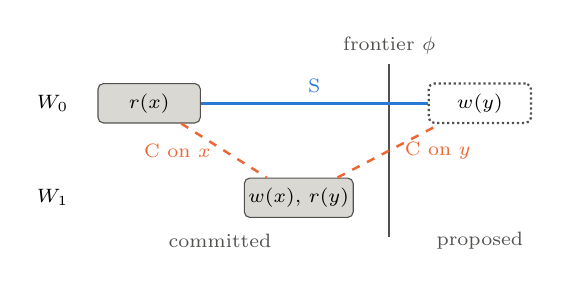
\begin{tikzpicture}[
  piece/.style={draw=ccmuted, rounded corners=2pt, minimum height=5mm,
                minimum width=13mm, font=\scriptsize, inner sep=1.5pt},
  done/.style={piece, fill=ccgrid},
  prop/.style={piece, densely dotted, line width=0.8pt},
  S/.style={ccblue, line width=0.9pt},
  C/.style={ccorange, line width=0.9pt, dashed},
  lab/.style={font=\scriptsize}]
% timeline
\node[lab, anchor=east] at (-0.2,1.2) {$W_0$};
\node[lab, anchor=east] at (-0.2,0.0) {$W_1$};
\node[done] (p0) at (0.7,1.2) {$r(x)$};
\node[done] (q)  at (2.6,0.0) {$w(x),\,r(y)$};
\node[prop] (p1) at (4.9,1.2) {$w(y)$};
\draw[ccmuted, line width=0.6pt] (3.75,1.7) -- (3.75,-0.5);
\node[lab, ccmuted, anchor=south] at (3.75,1.7) {frontier $\phi$};
\node[lab, ccmuted] at (1.6,-0.55) {committed};
\node[lab, ccmuted] at (4.9,-0.55) {proposed};
% edges
\draw[S] (p0) -- (p1) node[midway, above, lab, ccblue] {S};
\draw[C] (p0) -- (q)  node[midway, left=1pt, lab, ccorange] {C on $x$};
\draw[C] (q)  -- (p1) node[midway, right=2pt, lab, ccorange] {C on $y$};
\end{tikzpicture}
\caption{The impossibility witness of Corollary~\ref{cor:imp}. $W_0$ has
committed a read of $x$; $W_1$ has committed a piece that wrote $x$ and read
$y$. $W_0$ now proposes to write $y$. The cycle is mixed and passes through
$W_0$'s committed read. $W_0$'s remainder is already a single piece, so there
is nothing left to merge, and $W_1$ having finished does not remove its
edges.}
\label{fig:witness}
\end{figure}

\paragraph{Waiting does not help.}
The practically important part of Corollary~\ref{cor:imp} is that the refusal
cannot be waited out. One might hope that letting all other workflows finish
would dissolve the conflict. It does not. A workflow that has fully committed
still contributes its S~clique and its C~edges, because those interleavings
really happened. Figure~\ref{fig:witness} shows the smallest instance: $W_1$
is finished, $W_0$'s remainder is a single piece, and the cycle is still
there. The schedule it stands for is a real anomaly---$W_0$ read $x$ before
$W_1$ wrote it, so $W_0$ precedes $W_1$; $W_1$ read $y$ before $W_0$ writes
it, so $W_1$ precedes $W_0$. The runtime's options are to refuse the revision
or to run a compensating action for the committed prefix, which is an
application-level obligation rather than a graph property.

\subsection{Admission must be serialized}

\begin{theorem}[Serialized admission]
\label{thm:serial}
Two revisions that are each admissible against a common plan snapshot may be
jointly inadmissible. Admission decisions must therefore be evaluated and
installed one at a time against a single plan snapshot.
\end{theorem}

\begin{proof}
By counterexample. $W_0$ has committed a read of $x$ and $W_1$ a read of $y$.
$W_0$ proposes to write $y$ and $W_1$ proposes to write $x$. Against the
common snapshot, each revision alone adds one C~edge and creates no cycle, so
each is admitted. Applied together, the plan contains the cycle
$r_0(x)$--$w_0(y)$--$r_1(y)$--$w_1(x)$--$r_0(x)$, which alternates S and
C~edges, and the plan admits a non-serializable execution.
\end{proof}

The runtime therefore evaluates and installs revisions under a single
admission lock, which also fixes the frontier used for sealing. A piece that
is currently executing is treated as immutable, exactly like a committed one,
so that a concurrent admission cannot regroup a piece another thread is
running.

\subsection{The admission algorithm}

\begin{algorithm}[t]
\caption{Admitting a plan revision}
\label{alg:admit}
\begin{algorithmic}[1]
\Require current plan $P$, frontier $\phi$, proposed revision of workflow $r$
\Ensure an installed plan, or a refusal with a witness cycle
\State \textbf{acquire} the admission lock \Comment{Theorem~\ref{thm:serial}}
\State $P' \gets P$ with $r$'s uncommitted suffix replaced
\If{$P'$ is SC-cycle-free}
  \State \Return \textsc{Admit}$(P')$ \Comment{finest plan, unchanged}
\EndIf
\State $S \gets \seal(P',\phi)$
\If{$S$ has a mixed simple cycle $c$}
  \State \Return \textsc{Refuse}$(c)$ \Comment{Corollary~\ref{cor:imp}}
\EndIf
\Repeat \Comment{guided coarsening, suffix only}
  \ForAll{mixed biconnected blocks $b$ of $P'$}
    \State pick a workflow $w$ with an S~edge in $b$ beyond $\phi(w)$
    \State merge the interval of $w$ whose merge adds the least
      footprint~$\times$~duration
  \EndFor
\Until{$P'$ is SC-cycle-free}
\State \Return \textsc{AdmitCoarsened}$(P')$
\end{algorithmic}
\end{algorithm}

Algorithm~\ref{alg:admit} proceeds in three steps. It first certifies the
proposed plan as given, because when the proposal already certifies we want
the finest plan, not the coarsest. If that fails it tests the sealing; by
Theorem~\ref{thm:char} a failure here is final, and the algorithm returns the
witness cycle and the workflows it implicates so that the application can
choose compensation or an alternative plan. Otherwise it runs a guided
coarsening restricted to pieces at or beyond the frontier. Each pass repairs
every mixed block and chooses, per workflow, the merge that adds the least
footprint-duration area, a proxy for how much additional lock holding the
merge causes. Each pass strictly reduces the number of pieces, so the loop
terminates, and by Theorem~\ref{thm:char} it must succeed once the sealing has
certified.

The same algorithm with an empty frontier is the launch-time certifier: it
takes the finest chopping the agents declare and returns the finest plan it
can certify.

\section{Runtime}
\label{sec:runtime}

The certificate of \S\ref{sec:theory} is conditional on the execution rules
E1--E4. The job of the runtime is to make those hypotheses true. It sits
between the agents and the target system as a middleware: every tool call an
agent emits is dispatched through it, and nothing reaches the target system
any other way. Figure~\ref{fig:arch} shows the path of a call.

\begin{figure}[t]
\centering
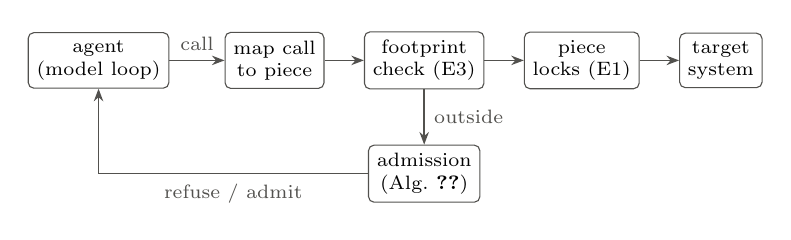
\begin{tikzpicture}[
  box/.style={draw=ccmuted, rounded corners=2pt, font=\scriptsize,
              minimum height=6mm, inner sep=3pt, align=center},
  arr/.style={-{Stealth[length=1.6mm]}, ccmuted, line width=0.6pt},
  lab/.style={font=\scriptsize, ccmuted}]
\node[box] (agent) at (0,0) {agent\\(model loop)};
\node[box, right=7mm of agent] (piece) {map call\\to piece};
\node[box, right=5mm of piece] (enf) {footprint\\check (E3)};
\node[box, right=5mm of enf] (lock) {piece\\locks (E1)};
\node[box, right=5mm of lock] (store) {target\\system};
\node[box, below=7mm of enf] (adm) {admission\\(Alg.~\ref{alg:admit})};
\draw[arr] (agent) -- node[above, lab] {call} (piece);
\draw[arr] (piece) -- (enf);
\draw[arr] (enf) -- (lock);
\draw[arr] (lock) -- (store);
\draw[arr] (enf) -- node[right, lab] {outside} (adm);
\draw[arr] (adm.west) -| node[pos=0.25, below, lab] {refuse / admit} (agent.south);
\end{tikzpicture}
\caption{The path of one tool call. A call inside the footprint of the
executing piece proceeds to locking. A call outside it is a plan revision: it
is admitted, possibly after coarsening, or refused and reported back to the
agent as a tool result.}
\label{fig:arch}
\end{figure}

\subsection{Mediation and fail-closed enforcement}

Every read, range scan and write is checked against the footprint of the
piece that is currently executing for that workflow. An access inside the
footprint proceeds. An access outside it never reaches the target system.
Instead it is treated as what it is, a proposal to revise the plan, and is
handed to Algorithm~\ref{alg:admit}. If the revision is admitted the plan is
updated and the call proceeds; if it is refused the call fails, and the agent
receives the refusal as the result of its tool call.

Enforcement does not depend on the agent's cooperation. This matters because
a model-driven agent does not follow a script: it can call any tool with any
argument at any time, and its own account of what it intends to do is not
evidence. The trust boundary is explicit. The tools and the middleware are
trusted; the agent that drives them is not.

\paragraph{Pieces for a model-driven agent.}
A scripted workflow declares its steps and their grouping directly. A
model-driven agent declares only a footprint per piece, and the runtime must
decide which piece a call belongs to. It advances from the piece currently
held to the first later piece whose footprint permits the access; if none
does, the access stays with the current piece and becomes a revision proposal.
Every gap between two tool calls of a model-driven agent is a reasoning gap,
so a piece that certification left unmerged closes when its call returns. A
piece that certification merged across a reasoning gap is held through it;
releasing it per call would undo exactly the repair that made the plan safe.

\subsection{Piece isolation: three locking disciplines}
\label{sec:runtime:locking}

Rule E1 requires each piece to be serializable with respect to every other
piece. We enforce it by locking, with read and write modes and with range
locks so that an insert into a scanned range is blocked. Locks never outlive a
piece: they are released when the piece commits, which is what lets a chopped
workflow give up its shared footprint before the model starts reasoning.

Within that frame there is a design choice---when a piece acquires its
locks---and we study three answers (Table~\ref{tab:locking}).

\begin{table}[t]
\caption{Three ways to isolate a piece. All release at the piece boundary and
all run under the same certificate.}
\label{tab:locking}
\small
\begin{tabular}{@{}l>{\raggedright}p{2.05cm}>{\raggedright}p{1.85cm}>{\raggedright\arraybackslash}p{1.9cm}@{}}
\toprule
 & acquires & on conflict & aborts when \\
\midrule
\cc     & whole footprint, one wait & wait & never \\
\cctwo  & per access, at first use  & wait & a wait-for cycle is detected \\
\ccs    & per access, at first use  & higher $\sigma$ waits; lower $\sigma$ wounds & a lower-$\sigma$ piece needs the lock \\
\bottomrule
\end{tabular}
\end{table}

\paragraph{\cc: atomic footprint.}
A piece acquires locks for its entire declared footprint atomically, in one
wait, before executing. Because nothing is acquired while holding a lock, no
wait-for cycle can form and the lock manager is deadlock-free by
construction. The cost is over-reservation in time: an object the piece will
not touch until its last step is locked from its first step.

\paragraph{\cctwo: two-phase locking inside a piece.}
A piece takes each lock when the access happens and releases all of them
together at the piece boundary: strict two-phase locking scoped to a piece.
Holds are shorter, but hold-and-wait returns, and with it deadlock. The
typical case is a lock upgrade. Two pieces each hold a read lock on an object
and each then requests the write lock. \cctwo detects the cycle in the
wait-for graph, aborts the member with the highest $\sigma$, undoes its writes
through the registered inverses, and restarts it.

\paragraph{\ccs: priority-ordered locking.}
The deadlock in \cctwo is the only thing standing between incremental locking
and a strict improvement, and it does not have to be detected. It can be made
unreachable. The device is the one \mtpo uses for notifications: a rank
$\sigma$ assigned to every workflow at launch, and a rule that influence flows
in one direction along it. Applied to lock waits, the rule is:
\begin{itemize}
\item if the requester's $\sigma$ is \emph{higher} than the holder's, the
  requester \emph{waits};
\item if the requester's $\sigma$ is \emph{lower} than the holder's, the
  holder is \emph{wounded}: it is aborted, its writes are undone, its locks
  are released, and the requester proceeds.
\end{itemize}
This is the wound-wait scheme of Rosenkrantz et al.~\cite{rosenkrantz1978}
with $\sigma$ as the timestamp. We chose it over wait-die because wait-die
aborts a requester the moment it meets any held lock, including one about to
be released.

The semantics line up with \mtpo as well. Under \mtpo the lower-ranked agent
writes as though it ran first and the higher-ranked agent absorbs the change
through a notification. Under \ccs the lower-ranked agent takes the lock as
though it ran first and the higher-ranked agent absorbs the change by aborting
and redoing. The order is the same and the direction of yielding is the same;
what differs is the mechanism of the yield---premise repair there, redo here.
\S\ref{sec:eval:agent} shows that this difference matters for agents.

\begin{proposition}[The certificate survives incremental locking]
\label{prop:atomic}
Under \cctwo and \ccs, every execution satisfies E1.
\end{proposition}

\begin{proof}
Both disciplines acquire a lock before each access and release no lock before
the piece commits or aborts, and an aborted piece's writes are undone before
its locks are released. This is strict two-phase locking with pieces as the
transactions, so the execution is conflict-serializable at piece granularity
and no piece observes an uncommitted write of another.
\end{proof}

One-shot acquisition was therefore never buying correctness. It was buying
deadlock freedom, and \ccs buys that differently:

\begin{proposition}[\ccs is deadlock-free]
\label{prop:acyclic}
Under \ccs the wait-for graph is acyclic at all times.
\end{proposition}

\begin{proof}
A workflow waits only for a workflow of strictly lower $\sigma$. A cycle in
the wait-for graph would require $\sigma$ to decrease strictly around the
cycle, which is impossible.
\end{proof}

The workflow with the lowest $\sigma$ never waits and is never wounded, so
some workflow always makes progress. A higher-ranked workflow can be wounded
repeatedly; the runtime caps restarts and reports a workflow that exhausts the
cap as failed. We measure how often wounds occur and whether the cap is ever
reached in \S\ref{sec:eval:locking}.

\subsection{Refusals, aborts and the agent}

Two runtime events are visible to the agent, and they ask different things of
it.

A \emph{refusal} is returned as the result of the offending tool call. The
agent's conversation is intact, and it is expected to continue: by retrying
once the blocking piece has released, by choosing an operation inside its
footprint, or by reporting that the intent cannot be met.

An \emph{abort}---a deadlock victim under \cctwo or a wound under
\ccs---restarts the agent. Its writes are undone, its locks are released, and
its conversation is reset to the original task statement. The agent does not
see a partial failure and is not asked to reason about one; it performs its
task again against the current state.

\subsection{Durable continuation}

Chopping trades failure atomicity for concurrency: once a piece commits, its
effects are visible even if the process dies before the next piece. The
certificate says nothing about this, and the runtime must. Each piece's writes
and the workflow's progress record, including its local variables, are
committed in one transaction of the underlying store. A crash inside that
transaction rolls back both, so pieces are atomic; a crash after it leaves a
durable marker from which recovery replays the remaining pieces forward (rule
E4).

\subsection{Implementations}
\label{sec:runtime:impl}

We built the mechanism twice. The \emph{durable runtime} is about 1{,}470
lines of Python over SQLite in write-ahead-logging mode. It runs workflows on
real threads, implements \cc with durable continuation, and is used for the
mechanism-level throughput, crash and certification-cost experiments.

The \emph{agent runtime} is a middleware in the style of
CoAgent~\cite{lyu2026coagent}: tools declare footprints and register
inverses, and a concurrency-control protocol is consulted on every call. In
it we implemented \cc, \cctwo and \ccs next to five other protocols---serial
execution, no coordination, whole-workflow 2PL and OCC with saga undo, and
\mtpo---so that all eight face the same agents, tools and workloads. Its
store is in memory, so it has no crash boundary and does not implement durable
continuation. An abort in this runtime restarts the whole workflow and
compensates the writes of pieces it had already committed, rather than
restarting only the aborted piece from a progress record; \S\ref{sec:discussion}
discusses the consequence.

\section{Verification}
\label{sec:verification}

Every soundness claim in \S\ref{sec:theory} is checked by brute force rather
than argued only on paper. The ground truth is an oracle that enumerates every
interleaving of the pieces of a plan that respects program order, builds the
conflict graph at workflow granularity for each, and tests it for cycles. A
plan is \emph{truly safe} if and only if no interleaving has a cyclic graph.
The certifier is sound if it never certifies a plan the oracle finds unsafe.

\begin{table}[t]
\caption{Bounded exhaustive verification of the durable runtime. Ground truth
enumerates executions and tests conflict-serializability at workflow
granularity.}
\label{tab:verify}
\small
\begin{tabular}{@{}p{3.55cm}rp{1.85cm}r@{}}
\toprule
Property checked & Scale & Ground truth & Viol. \\
\midrule
Static certification, 2 workflows & 256 plans & all interleavings & 0 \\
Static certification, 3 workflows & 4{,}096 plans & all interleavings & 0 \\
Repair yields a serial-equivalent plan & 3{,}820 repairs & all interleavings & 0 \\
Cycles persist under refinement (Lemma~\ref{lem:persist}) & 1{,}023 refin. & 258 sealed cycles & 0 \\
Admission soundness (Theorem~\ref{thm:inherit}) & 3{,}000 revisions & all interleavings & 0 \\
Committed prefix never rewritten & 3{,}000 revisions & structural equality & 0 \\
Sealing characterization (Theorem~\ref{thm:char}) & 9{,}290 choppings & exhaustive future-only search & 0 \\
Range footprints catch phantoms & 2{,}000 scenarios & all interleavings & 0 \\
Concurrent runtime, safe policies & 72 batches & trace oracle + invariants & 0 \\
Unchecked control must fail & 18 batches & trace oracle + invariants & 0 \\
\bottomrule
\end{tabular}
\end{table}

Table~\ref{tab:verify} summarizes the checks. Static certification is
exhaustive over all assignments of read and write to two shared items across
two and three workflows: every plan is either certified and checked against
all interleavings, or rejected, repaired, and then checked against all
interleavings of the repaired plan. Prefix-aware admission is checked on
3{,}000 randomly generated revision scenarios with randomly placed frontiers.
For each we confirm that an admitted plan is serial-equivalent under every
interleaving and that the committed prefix was never rewritten. By enumerating
all 9{,}290 future-only choppings across those scenarios we confirm that
refusal coincides exactly with the non-existence of a certified future-only
coarsening, which is Theorem~\ref{thm:char}. The refinement row is
non-vacuous by construction: it counts only scenarios whose sealing fails to
certify.

Two constructed witnesses are machine-checked as well: the impossibility
instance of Figure~\ref{fig:witness}, where the single available future-only
chopping fails to certify and the plan admits a non-serializable execution,
and the concurrent-admission counterexample of Theorem~\ref{thm:serial}.

The verifier also drives the concurrent runtime, not only the graph logic. It
runs batches of 16 workflows at eight threads with mid-flight revisions in
progress and requires every recorded history to be serializable and every
application invariant to hold. It separately requires that the
\emph{unchecked} control---the same fine chopping executed with no
certification---does fail, so that a passing run cannot be an artefact of
undemanding workloads.

\paragraph{Independent re-implementation.}
The agent runtime of \S\ref{sec:runtime:impl} re-implements certification,
sealing, admission and guided coarsening from the definitions, without sharing
code with the durable runtime, and is checked against its own brute-force
oracle: exhaustive static plans for two workflows over two items and three
workflows over one, 300 repaired plans, 400 refinement scenarios, 250 characterization scenarios compared with
exhaustive future-only search, 300 admitted revisions, both witnesses, a
phantom scenario and a fail-closed enforcement test. All pass. Two independent
implementations agreeing with two independent oracles does not prove the
theorems, but it makes a shared implementation error an unlikely explanation
for the results.

\paragraph{Scope.}
These results are bounds, not proofs of unbounded correctness. They cover
small batches, a two-item alphabet for the static sweep, and syntactic
read/write conflicts. They do not establish that real tool footprints are
sound, which is an assumption the runtime enforces but cannot originate.

\section{Evaluation}
\label{sec:eval}

We evaluate with two instruments. The \emph{agent study}
(\S\ref{sec:eval:setup}--\S\ref{sec:eval:revisions}) drives every protocol
with real language-model agents and answers four questions:
\begin{description}
\item[RQ1] Does certified chopping prevent the anomalies that uncoordinated
  agents produce, and how does it compare with locking and with repair?
\item[RQ2] What does it cost in time and tokens?
\item[RQ3] How do the three locking disciplines of
  \S\ref{sec:runtime:locking} differ?
\item[RQ4] How much does each protocol's correctness depend on the model?
\end{description}
The \emph{mechanism study} (\S\ref{sec:eval:mechanism}) uses the durable
runtime with real threads and a calibrated reasoning delay to measure
throughput at higher concurrency, admission rates under controlled
contention, certification cost and crash recovery.

\subsection{Agent study: setup}
\label{sec:eval:setup}

\paragraph{Workloads.}
Each workload, which we call a \emph{cell}, gives two agents natural-language
tasks over a small shared state and a set of tools. Table~\ref{tab:cells}
lists the twelve cells. Ten are \emph{contended}: they follow the methodology
of CoAgent's contended cells~\cite{lyu2026coagent}, with operations drawn from
cloud operations in the style of AIOpsLab~\cite{chen2025aiopslab} and
workplace tasks in the style of WorkBench~\cite{styles2024workbench}, and
each is built so that an unlucky interleaving produces a specific anomaly.
Two are structural cells for chopping: \cell{cc-claim} has a short shared
dependency followed by private work, the shape of
Figure~\ref{fig:sc}(a), and \cell{cc-escalate} is the impossibility witness of
Figure~\ref{fig:witness} made executable.

\begin{table}[t]
\caption{The twelve cells. Each runs two concurrent agents.}
\label{tab:cells}
\small
\begin{tabular}{@{}lp{5.1cm}@{}}
\toprule
Cell & Anomaly an unlucky interleaving produces \\
\midrule
\cell{k8s-canary}            & stale read + missed range scan \\
\cell{k8s-port-misconfig}    & phantom insert + stale read \\
\cell{k8s-permission-revoke} & phantom insert + stale read \\
\cell{k8s-replica-scale}     & lost update \\
\cell{k8s-rollback-audit}    & non-idempotent append on a stale premise \\
\cell{wb-crm-dedupe}         & phantom insert + stale read \\
\cell{wb-calendar-doublebook}& lost update (double booking) \\
\cell{wb-email-triage}       & non-idempotent append on a stale premise \\
\cell{wb-analytics-restate}  & phantom insert + stale read \\
\cell{wb-project-rebalance}  & lost update \\
\midrule
\cell{cc-claim}              & none: short shared read, private work \\
\cell{cc-escalate}           & mid-flight escalation into a peer's committed footprint \\
\bottomrule
\end{tabular}
\end{table}

\paragraph{Protocols.}
All eight protocols run on the same middleware, tools and agents:
\textbf{Serial} (one agent at a time, the correctness and speed reference);
\textbf{Naive} (no coordination); \textbf{2PL} and \textbf{OCC}
(whole-workflow isolation with saga undo); \textbf{\mtpo}, our
re-implementation of CoAgent's protocol from its paper, since its code is not
public; and \cc, \cctwo and \ccs.

\paragraph{Agents and models.}
Agents are driven by Claude Haiku~4.5 with extended thinking, and by Claude
Sonnet~5 at low reasoning effort. The Haiku run covers all eight protocols;
the Sonnet run covers the six that existed when it was made, that is, all but
\cctwo and \ccs. Every (cell, protocol) pair is run for ten seeds: 962 trials
with Haiku and 720 with Sonnet, at a total API cost of \$24.89.

\paragraph{Time.}
The agent runtime is a discrete-event scheduler. The duration of each tool
call is the measured wall-clock latency of the model inference that produced
it, and an agent that is blocked waits on the same clock. The time of a trial
is its makespan on this clock. \emph{Speedup} for a cell is the median serial
time divided by the median protocol time; we use medians because a single
trial with a stuck agent moves a mean by orders of magnitude. Aggregate
speedup is the mean over cells.

\paragraph{Scoring.}
For each cell we compute the set of final states that the two serial orders
can produce. A trial is \emph{anomaly-free} if the part of its final state
that concurrency can corrupt matches one of them; for \cell{cc-escalate}, a
refused escalation that leaves the shared state untouched is anomaly-free,
because refusing is the mechanism working. This predicate deliberately ignores
errors an agent makes on its own, which we measure separately as assumption A1
(\S\ref{sec:eval:agent}).

The predicate is trustworthy only if serial execution always satisfies it.
With Haiku, serial execution fails it on \cell{k8s-rollback-audit} (5/10) and
\cell{wb-email-triage} (9/10): the model alone gets the record format wrong
often enough that an agent error is indistinguishable from an anomaly. We
show these two cells but exclude them from Haiku aggregates, leaving ten
scored cells. With Sonnet, serial execution passes every cell and all twelve
are scored.

\paragraph{Statistics.}
Proportions carry 95\% Wilson intervals~\cite{wilson1927}. Speed differences
between protocols are paired by cell and carry 95\% bootstrap intervals over
cells (20{,}000 resamples).

\subsection{RQ1: Safety}
\label{sec:eval:safety}

\begin{table*}[t]
\caption{Anomaly-free trials per cell with Claude Haiku~4.5 (out of 10 unless
noted). Cells marked $\dagger$ are excluded from the total because serial
execution itself fails their predicate.}
\label{tab:percell}
\small
\begin{tabular}{@{}lrrrrrrrr@{}}
\toprule
Cell & Serial & Naive & 2PL & OCC & \mtpo & \cc & \cctwo & \ccs \\
\midrule
\cell{k8s-canary}             & 10 & 6 & 10 & 5 & 10 & 10 & 10 & 10 \\
\cell{k8s-port-misconfig}     & 10 & 4 & 10 & 7 & 10 & 8 & 8 & 9 \\
\cell{k8s-permission-revoke}  & 10 & 9 & 10 & 10 & 10 & 10 & 10 & 10 \\
\cell{k8s-replica-scale}      & 10 & \textbf{0} & 10 & 10 & \textbf{6} & 10 & 10 & 10 \\
\cell{wb-crm-dedupe}          & 10 & 9 & 8 & 10 & 10 & 9 & 9 & 10 \\
\cell{wb-calendar-doublebook} & 10 & \textbf{0} & 10 & 9 & 9 & 10 & 10 & 10 \\
\cell{wb-analytics-restate}   & 10 & 8 & 10 & 9 & 10 & 10 & 10 & 10 \\
\cell{wb-project-rebalance}   & 10 & \textbf{0} & 8 & 8 & 8 & 9 & 10 & 9 \\
\cell{cc-claim}               & 10 & 10 & 10 & 10 & 10 & 10 & 9 & 10 \\
\cell{cc-escalate}            & 10 & 10 & 10 & 10 & 10 & 10 & 10 & 10 \\
\midrule
\textbf{Total (10 cells)}     & 100 & 56 & 96 & 88 & 93 & 96 & 96 & \textbf{98} \\
\midrule
\cell{k8s-rollback-audit}$^\dagger$ & 5 & 7 & 4 & 3 & 5/11 & 6 & 5 & 4 \\
\cell{wb-email-triage}$^\dagger$    & 9 & 7 & 8 & 6 & 5/11 & 10 & 6 & 8 \\
\bottomrule
\end{tabular}
\end{table*}

\begin{figure*}[t]
\centering
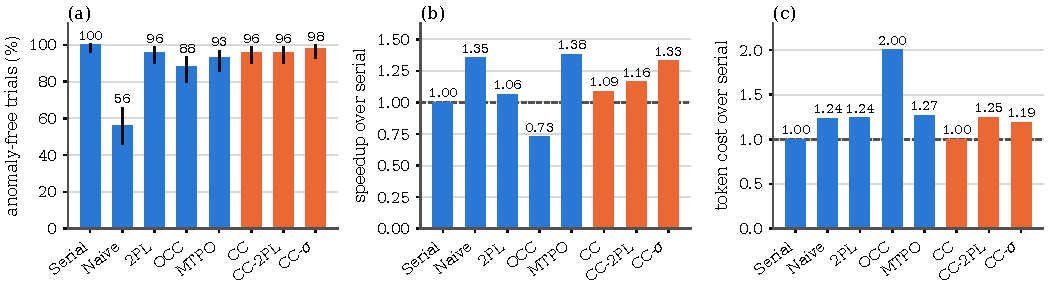
\includegraphics[width=\textwidth]{figs/main_haiku.pdf}
\caption{Claude Haiku~4.5. (a)~Anomaly-free trials over the ten scored cells,
with 95\% Wilson intervals. (b)~Mean speedup over serial execution and
(c)~mean token cost relative to serial, both over the eight contended scored
cells, on which every protocol performs the same work. Orange bars are the
certified-chopping variants.}
\label{fig:main}
\end{figure*}

Table~\ref{tab:percell} and Figure~\ref{fig:main}(a) show the Haiku results.

\paragraph{Uncoordinated agents fail, and fail structurally.}
Naive execution is anomaly-free in 56\% of trials. The three lost-update cells
fail in \emph{every} trial (0/10 each), with both models. A lost update does
not need unlucky timing: both agents must read before they write, so the
window is always open.

\paragraph{Certified chopping matches locking and exceeds repair.}
All three chopping variants are at least as safe as whole-workflow 2PL
(96\%): \cc and \cctwo at 96\% and \ccs at 98\% $[93, 99]$. \mtpo is at 93\%
$[86, 97]$. The intervals overlap, and we do not claim the differences among
the safe protocols are significant at this sample size. What the table does
show is \emph{where} each protocol loses trials. \mtpo's losses are
concentrated: 6/10 on \cell{k8s-replica-scale}, the cell where its correctness
depends on the notified agent recomputing its write. On that cell the three
chopping variants score 10/10 each, because certification merged the
read-modify-write into one piece and the interleaving \mtpo must repair never
occurs. The remaining failures of the locking-based protocols, chopping
included, are spread thinly (one or two trials on a few cells). Their final
states are not interleavings: one agent's work is missing or incomplete---an
ingress never created, one of two updates absent. Whole-workflow 2PL, which
cannot interleave at all, loses trials on the same cells in the same way. We
attribute these to the agent rather than the protocol; this model completes
its task correctly in only 78\% of trials even when run alone
(\S\ref{sec:eval:agent}).

\paragraph{A stronger model.}
With Sonnet, serial execution is correct in all 120 trials, which removes the
individual-error confound. On the ten contended cells \cc is anomaly-free in
100/100 trials, against 96/100 for 2PL, 95/100 for \mtpo and 93/100 for OCC.
\mtpo's failures are again concentrated on a repair obligation: 7/10 on
\cell{k8s-rollback-audit}, examined in \S\ref{sec:eval:agent}. \cc's only
Sonnet failures are three trials of \cell{cc-claim}, also examined there, for
an overall 117/120 (98\% $[93, 99]$).

\subsection{RQ2: Speed and cost}
\label{sec:eval:speed}

\begin{table}[t]
\caption{Aggregate results. AF: anomaly-free trials over all scored cells (10
for Haiku, 12 for Sonnet), as is cost per trial. Speedup and token cost are
relative to serial execution over the contended scored cells (8 for Haiku, 10
for Sonnet). Worst: the slowest such cell.}
\label{tab:agg}
\small
\begin{tabular}{@{}lrrrrr@{}}
\toprule
 & AF (\%) & Speedup & Worst & Tokens & \$/trial \\
\midrule
\multicolumn{6}{@{}l}{\emph{Claude Haiku~4.5}} \\
Serial   & 100 & 1.00 & 1.00 & 1.00 & 0.0124 \\
Naive    & 56  & 1.35 & 0.93 & 1.24 & 0.0150 \\
2PL      & 96  & 1.06 & 0.86 & 1.24 & 0.0147 \\
OCC      & 88  & 0.73 & 0.50 & 2.00 & 0.0240 \\
\mtpo    & 93  & \textbf{1.38} & 0.86 & 1.27 & 0.0150 \\
\cc      & 96  & 1.09 & 0.70 & \textbf{1.00} & 0.0125 \\
\cctwo   & 96  & 1.16 & 0.83 & 1.25 & 0.0146 \\
\ccs     & \textbf{98} & 1.33 & \textbf{1.08} & 1.19 & 0.0141 \\
\midrule
\multicolumn{6}{@{}l}{\emph{Claude Sonnet~5}} \\
Serial   & 100 & 1.00 & 1.00 & 1.00 & 0.0120 \\
Naive    & 75  & 1.36 & 0.95 & 1.19 & 0.0145 \\
2PL      & 97  & 1.05 & 0.81 & 1.22 & 0.0145 \\
OCC      & 94  & 0.73 & 0.52 & 1.86 & 0.0219 \\
\mtpo    & 96  & \textbf{1.43} & \textbf{1.12} & 1.20 & 0.0146 \\
\cc      & \textbf{98}  & 1.01 & 0.93 & \textbf{1.01} & 0.0125 \\
\bottomrule
\end{tabular}
\end{table}

We report speed on the contended cells, where every protocol performs the
same work. The two structural cells are discussed separately below, because on
\cell{cc-escalate} the chopping variants refuse a write that the other
protocols perform, and a protocol should not be credited for finishing sooner
by doing less. (Including both structural cells, the Haiku means are
$1.48\times$ for \ccs and $1.47\times$ for \mtpo.)

\paragraph{Contended cells.}
Figure~\ref{fig:main}(b) and Table~\ref{tab:agg} show the result. Plain \cc is
barely faster than serial ($1.09\times$ with Haiku, $1.01\times$ with Sonnet)
and no faster than 2PL. This is the expected, honest outcome. Every contended
cell has a read-modify-write or a scan-then-insert straddling the reasoning
gap, so certification merges each workflow into one piece at launch---it does
so in every trial on all ten contended cells---and the policy \emph{is}
whole-workflow locking. Certified chopping bought nothing there, and it is
important that it bought nothing rather than buying speed unsafely.

The locking discipline changes the picture. \ccs reaches $1.33\times$,
statistically indistinguishable from \mtpo's $1.38\times$
(Table~\ref{tab:boot}), and significantly faster than both 2PL and plain \cc
on every one of the eight cells. It is also the only protocol in the Haiku
run whose slowest cell is still faster than serial ($1.08\times$); 2PL and
\mtpo both bottom out at $0.86\times$ and plain \cc at $0.70\times$.

\begin{table}[t]
\caption{Paired speedup differences on the eight contended scored cells
(Haiku), with 95\% bootstrap intervals over cells and the number of cells on
which the first protocol is faster/slower.}
\label{tab:boot}
\small
\begin{tabular}{@{}lrcr@{}}
\toprule
Comparison & Mean diff. & 95\% CI & +/-- \\
\midrule
\ccs $-$ \cc     & $+0.24$ & $[+0.16, +0.33]$ & 8/0 \\
\ccs $-$ 2PL     & $+0.27$ & $[+0.17, +0.36]$ & 8/0 \\
\ccs $-$ \cctwo  & $+0.17$ & $[+0.08, +0.25]$ & 6/2 \\
\ccs $-$ \mtpo   & $-0.05$ & $[-0.29, +0.19]$ & 3/5 \\
\cctwo $-$ \cc   & $+0.08$ & $[+0.02, +0.12]$ & 5/3 \\
\cc $-$ 2PL      & $+0.03$ & $[-0.09, +0.15]$ & 3/5 \\
\bottomrule
\end{tabular}
\end{table}

\paragraph{Where chopping pays.}
On \cell{cc-claim} the certificate keeps the cut, the lock on the shared pool
is released before either agent reasons, and all work is performed (with
Haiku, every trial of every protocol completes both agents' writes). 2PL is
no faster than serial there ($0.98\times$). \cc reaches $1.73\times$, \cctwo
$1.87\times$ and \ccs $2.15\times$, against \mtpo's $1.79\times$. This is the
structure chopping exists for: the shared dependency is short and the private
interval is long.

\paragraph{Tokens.}
Figure~\ref{fig:main}(c) shows token cost. Plain \cc costs the same as serial
execution ($1.00\times$): it never aborts and never notifies, so no inference
is repeated and no context is added. \ccs costs $1.19\times$, below 2PL
($1.24\times$) and \mtpo ($1.27\times$). The two faster protocols pay in
different currencies, which Table~\ref{tab:mech} separates: \ccs runs more
rounds than \mtpo (8.2 against 7.7 per trial) because wounded agents redo
work, but \mtpo spends more tokens in total (7{,}339 against 6{,}810)
because every notification adds its payload, and the reasoning about it, to
the agent's context.

\subsection{RQ3: Locking disciplines}
\label{sec:eval:locking}

\begin{table}[t]
\caption{Mechanism counts per trial over the ten scored cells (Haiku),
recovered from runtime traces.}
\label{tab:mech}
\small
\begin{tabular}{@{}lrrrrrr@{}}
\toprule
 & Deadl. & Wounds & Aborts & Notif. & Rounds & Tokens \\
\midrule
Serial & 0 & 0 & 0 & 0 & 6.9 & 6{,}104 \\
2PL    & 0.76 & 0 & 0.76 & 0 & 8.5 & 7{,}077 \\
\mtpo  & 0 & 0 & 0 & 0.80 & 7.7 & 7{,}339 \\
\cc    & 0 & 0 & 0 & 0.10 & 7.1 & 6{,}245 \\
\cctwo & 0.80 & 0 & 0.80 & 0.10 & 8.6 & 7{,}076 \\
\ccs   & 0 & 0.78 & 0.78 & 0.10 & 8.2 & 6{,}810 \\
\bottomrule
\end{tabular}
\end{table}

\begin{figure}[t]
\centering
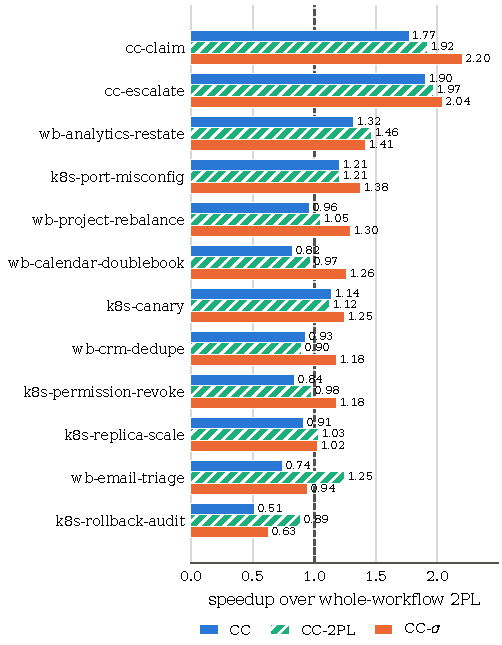
\includegraphics[width=\columnwidth]{figs/percell_haiku.pdf}
\caption{Speedup of each locking discipline over whole-workflow 2PL, per cell
(Haiku, all twelve cells). On the dashed line a protocol is no better than
2PL. \ccs trails 2PL only on the two cells at the bottom, which are the two
contended cells on which 2PL never deadlocks.}
\label{fig:percell}
\end{figure}

Table~\ref{tab:mech} and Figure~\ref{fig:percell} compare the three
disciplines.

\paragraph{Deadlock is the common case for incremental locking.}
\cctwo deadlocks 0.80 times per trial, slightly more often than
whole-workflow 2PL (0.76). The cause is the lock-upgrade pattern: both agents
read an object and both then try to write it. \cc never deadlocks, by
construction, and \ccs never deadlocks, by Proposition~\ref{prop:acyclic}; we
observed zero deadlocks in 120 trials of each.

\paragraph{Prevention beats detection.}
\ccs aborts as often as \cctwo (0.78 wounds against 0.80 deadlock aborts per
trial) and yet is significantly faster ($+0.17\times$,
Table~\ref{tab:boot}). The difference is \emph{when} the abort happens. A
wound is issued at the moment of conflict. A deadlock is resolved only after
both agents have blocked and the cycle has been found, and each has by then
spent a model inference producing the call on which it blocked.

We had expected aborts to be expensive to undo. They were not: all 76 deadlock
aborts of 2PL and all 80 of \cctwo, and 86 of the 90 wounds of \ccs, undid
zero writes. In these workloads the victim has read but not yet written, so
the cost of an abort is the repeated inference, not the compensation.

\paragraph{No starvation observed.}
The restart cap was never reached. Of the 100 scored \ccs trials, 78 contained
a wound, and all 78 ended anomaly-free; the two \ccs failures occurred in
trials with no wound.

\paragraph{Where \ccs loses: wounding without a deadlock to prevent.}
Figure~\ref{fig:percell} shows \ccs ahead of plain \cc on all twelve cells and
ahead of 2PL on ten. The two exceptions, \cell{wb-email-triage}
($0.94\times$) and \cell{k8s-rollback-audit} ($0.63\times$), follow an exact
rule. Across the twelve cells, 2PL deadlocks at a mean rate of 0.76 per trial
on the ten cells where \ccs beats it, and \emph{never} on the two where \ccs
loses. On those two cells contention is mild: 2PL resolves it by a short wait
and no abort. Wound-wait cannot tell a conflict that would have resolved
itself from one that would have deadlocked. It aborts the lower-priority
holder either way and so converts a short wait into a redo. \cctwo, which
aborts only on an actual cycle, is the fastest of the three disciplines on
exactly these two cells ($1.25\times$ and $0.89\times$). The two cells are the ones excluded
from Haiku aggregates, so this cost does not appear in Table~\ref{tab:agg}; we
report it here because it identifies the next refinement, discussed in
\S\ref{sec:discussion}.

\subsection{RQ4: Dependence on the agent}
\label{sec:eval:agent}

\begin{table}[t]
\caption{The two agent assumptions behind repair-based concurrency control,
measured. A1: serial trials whose final state exactly matches a reference.
A3: \mtpo trials with a notification that end anomaly-free.}
\label{tab:assump}
\small
\begin{tabular}{@{}lrr@{}}
\toprule
 & A1 (individual success) & A3 (self-healing) \\
\midrule
Assumed in~\cite{lyu2026coagent} & 98\% & 95\% \\
Claude Haiku~4.5 & 78\% & 71/78 = 91\% $[83, 96]$ \\
Claude Sonnet~5  & 100\% & 95/100 = 95\% $[89, 98]$ \\
\bottomrule
\end{tabular}
\end{table}

Every protocol depends on the agent for something. The question is for what,
and what happens when the agent falls short.

\paragraph{A1 moves with the model; A3 barely does.}
Table~\ref{tab:assump} measures the two assumptions. Individual success rises
from 78\% to 100\% between the two models. Self-healing rises only from 91\%
to 95\%. The stronger model fixes nearly all of its individual errors but
remains about one time in twenty unable to discharge a repair obligation. To
the extent two models can show it, repair looks like a structural residual
rather than a capability gap that the next model closes.

\paragraph{How repair fails.}
\cell{k8s-rollback-audit} makes the residual concrete. Agent $A$ rolls a
deployment back and logs that it did; agent $B$ appends an audit record naming
the image it observed. Under \mtpo with Sonnet, $A$'s record lands first, $B$
is notified that the image changed, and $B$ must retract its record and file a
corrected one. In seven of ten trials it does. In two it appends a
\emph{second} record instead of replacing the first; an append has no
inverse, so the log is left with a duplicate that no serial order produces. In
one it ignores the notification and files the stale value. \cc scores 10/10 on
this cell with Sonnet: the read and the append are in one sealed piece, and no
notification is ever sent.

\paragraph{Certified chopping relocates the obligation.}
It would be wrong to conclude that certified chopping is independent of the
agent. Its obligation is elsewhere: an agent whose call is \emph{refused}
must carry on correctly. \cell{cc-claim} with Sonnet shows both the
obligation and a subtlety of model-driven plans. Agent $B$'s task is a blind
write to the shared pool followed by a private write, and its certified plan
has one piece for each. Sonnet, more cautious than the task requires, first
\emph{reads} the pool. That read is permitted by the footprint of the piece
that was certified for the write, so it runs, and the piece closes when the
call returns. The write that follows now needs a new piece. Together with the
committed one it would close a mixed cycle through the other agent's read of
the pool, so the revision is refused, correctly by
Corollary~\ref{cor:imp}. The model's improvisation spent the piece its plan
had been certified with.

What happens next is up to the agent. Sonnet read first in nine trials of
ten. In the tenth it wrote blind, as instructed, and both writes completed. In
six it proceeded to its private write, leaving the pool update undone. In three it treated the
refusal as terminal and stopped, leaving its private claim unwritten as well;
these are \cc's three Sonnet failures. With Haiku, which performs the blind
write as instructed, the same cell completes fully in every trial.

\paragraph{Fail-safe against fail-dirty.}
The two failure modes are not symmetric. When \mtpo's obligation is not met,
shared state is corrupted in a way the system cannot undo: a duplicate or
stale record in an append-only log. When certified chopping's obligation is
not met, shared state is clean and serializable but an intent is unfinished,
and a retry would still complete it. A refusal is also visible to the runtime,
which knows exactly which call it refused, whereas an unperformed repair
looks, from outside, like an agent that decided no repair was needed.

\paragraph{Redo is easier than repair.}
\ccs asks a third thing of the agent: after a wound, do the task again from
the beginning. With Haiku, all 78 wounded trials on the scored cells ended
anomaly-free, a 100\% success rate $[95, 100]$, where the same model
discharges \mtpo's repair obligation in 91\% of notified trials. The
difference is plausibly the kind of reasoning required. A wounded agent
receives its original task and a fresh context; it is not asked to work out
which of its past operations a change invalidates.

\subsection{Mid-flight revisions}
\label{sec:eval:revisions}

\begin{table}[t]
\caption{Outcomes of mid-flight revisions. Top: durable runtime, 220 revisions
per contention level over 10 seeds. Bottom: live agents under \cc.}
\label{tab:admit}
\small
\begin{tabular}{@{}lrrrrr@{}}
\toprule
 & Revisions & Admitted & Coarsened & Refused & Rate \\
\midrule
1 shared pool  & 220 & 10 & 0 & 210 & 4\% \\
2 shared pools & 220 & 20 & 0 & 200 & 9\% \\
4 shared pools & 220 & 37 & 0 & 183 & 17\% \\
8 shared pools & 220 & 73 & 9 & 138 & 37\% \\
\midrule
Haiku agents   & 10 & 0 & 0 & 10 & 0\% \\
Sonnet agents  & 32 & 6 & 0 & 26 & 19\% \\
\bottomrule
\end{tabular}
\end{table}

Table~\ref{tab:admit} reports what admission decided. In the durable runtime,
where workflows escalate into one of $k$ shared pools after committing a
prefix, between 4\% and 37\% of revisions are admissible, rising as contention
is spread over more pools. The rest are refused because the residual cycle
passes through a committed piece. No admitted revision produced a
non-serializable history or violated an invariant.

With live agents, revisions arise only on the two structural cells. Haiku
produces ten, all on \cell{cc-escalate}, the executable witness of
Figure~\ref{fig:witness}; all ten are refused, the shared item is untouched in
every trial, and the final state is serializable. That 0\% is a correctness
result on a cell built to be inadmissible, not an estimate of an admission
rate. Sonnet's additional reads generate more revisions, 32 across both
cells, of which six are admitted.

This is the most important limitation we measured. Prefix-aware
recertification decides the question correctly and cheaply and never admits an
unsafe revision, but the answer is frequently no.

\subsection{Mechanism study on a durable store}
\label{sec:eval:mechanism}

The agent study has two agents per cell and an in-memory store. The mechanism
study complements it with the durable runtime: 32 workflows per batch on 8
worker threads against SQLite, 4 shared pools, 10 seeds per configuration,
and real wall-clock time. Reasoning is a 50\,ms calibrated delay rather than
model inference, so these are mechanism measurements, not agent latencies.
The baselines are a whole-workflow database transaction, whole-workflow 2PL
over the union footprint, whole-workflow OCC with read validation and range
re-scan, and \emph{unchecked chopping}, which executes the fine pieces with no
certification and serves as an unsafe control. Correctness is judged by
recording every mediated operation and testing the workflow-level
serialization graph of the actual history for cycles.

\begin{table}[t]
\caption{Durable runtime: speedup over a whole-workflow database transaction
(makespan, 10 seeds). Last column: seeds in which unchecked chopping produced
a non-serializable history and violated the application invariant.}
\label{tab:durable}
\small
\begin{tabular}{@{}lrrrrr@{}}
\toprule
Workload & 2PL & OCC & \cc & Unchecked & Unsafe \\
\midrule
claim    & 3.19 & 2.99 & \textbf{7.35} & 7.24 & 0/10 \\
budget   & 3.06 & 2.90 & 3.10 & 7.18 & 10/10 \\
retail   & 3.11 & 2.93 & 3.07 & 7.41 & 10/10 \\
calendar & 3.13 & 2.92 & 3.07 & 7.34 & 10/10 \\
replan   & 5.11 & \textbf{7.61} & 7.14 & 7.58 & 0/10 \\
escalate & 3.04 & 4.51 & \textbf{6.24} & 5.91 & 10/10 \\
\bottomrule
\end{tabular}
\end{table}

\paragraph{Throughput.}
Table~\ref{tab:durable} shows the same two regimes as the agent study, at
sixteen times the concurrency. On \emph{claim}, certification keeps all 96
pieces: \cc is $7.35\times$ faster than a whole-workflow transaction and
$2.4\times$ faster than whole-workflow 2PL, and 95th-percentile latency falls
from 1.96\,s to 0.12\,s. On \emph{budget}, \emph{retail} and \emph{calendar},
which have a read-modify-write or scan-then-insert across the reasoning gap,
certification merges the pieces and \cc performs as whole-workflow locking
does, within seed-to-seed noise. Unchecked chopping is about $2.4\times$
faster still on those three workloads and is non-serializable, with a violated
invariant, in all ten seeds of each; on \emph{calendar} it double-books rooms
although each workflow's logic is individually correct. On \emph{escalate},
where two thirds of workflows revise their plan mid-flight, prefix-aware
admission gives $6.24\times$ against $3.04\times$ for 2PL, with no
violations. No safe policy produced a non-serializable history in any seed.

\paragraph{Sensitivity.}
The benefit tracks contention structure and available concurrency, not
reasoning time alone. On \emph{claim}, the speedup of \cc over
whole-workflow 2PL is $5.99\times$ with one shared pool and $1.30\times$ with
sixteen, where there is little contention to relieve; $0.99\times$ with one
worker thread and $3.12\times$ with sixteen. With zero reasoning time it is
$0.59\times$: chopping is a net loss when there is no private interval to
release a lock for, because each extra piece boundary costs a commit. On
\emph{budget} the ratio stays between $0.82\times$ and $1.06\times$
throughout, as it must, since certification always merges that workload back
to whole-workflow locking.

\paragraph{Certification cost.}
Static certification takes 28.5\,ms for 32 workflows (96 pieces) and 131\,ms
for 128 workflows (384 pieces); indexing conflict candidates and repairing
every mixed block per pass brought the latter down from 22\,s for a naive
all-pairs implementation. Readmission is cheaper, 0.6\,ms and 5.0\,ms at the
same sizes, because the frontier constrains the search. The cost is not
always worth paying: certifying \emph{budget} costs 35\,ms against a batch
that runs for 0.68\,s and purchases no speedup. A deployment should cache
certificates per program template and recertify only on structural change.

\paragraph{Crash and recovery.}
Three workflows each move 10 units between a private pair of accounts, in two
pieces. There are no cross-workflow conflicts, so certification accepts the
chopping: the batch is isolation-safe and still not failure-atomic. Killing
the process after a debit piece commits leaves one pair broken and the batch
total at 5{,}990 instead of 6{,}000. Without durable continuation the damage
is permanent. With it, recovery resumes the workflow from its progress record
and restores the total. A crash \emph{inside} a piece's transaction rolls back
the writes together with the progress record, confirming that pieces are
atomic.

\section{Discussion and Limitations}
\label{sec:discussion}

\paragraph{What a system designer should take away.}
The result we would emphasize is not a speedup. It is that the admissibility
question for mid-flight revisions has a clean answer, that the answer is often
no, and that no runtime cleverness changes it once effects are visible. This
argues for three design practices: declare contingent footprints before
committing anything; treat the first visible effect of a workflow as a
commitment boundary in agent design, not an implementation detail; and, where
neither is possible, provide compensation. The whole-workflow baselines avoid
the problem by reserving the conservative union footprint in advance, which is
precisely the cost chopping tries to avoid.

\paragraph{Improvisation consumes certified pieces.}
The \cell{cc-claim} result with Sonnet (\S\ref{sec:eval:agent}) exposes a
hazard specific to model-driven agents. The runtime infers which piece a call
belongs to, and a piece closes when its call returns. A model that inserts an
extra, harmless-looking read can therefore commit the piece its later write
was certified under and turn its own admissible plan into an inadmissible
one. Two mitigations follow directly. Footprints can distinguish ``may read''
from ``will write'', so that a read does not close a piece that still owes a
write. And the tool interface can expose the atomic operation the certificate
actually covers, such as a single read-modify-write call, instead of its
parts.

\paragraph{Refining priority-ordered locking.}
\ccs pays for deadlock freedom on every conflict with a lower-priority holder,
including conflicts that would have resolved by a short wait
(\S\ref{sec:eval:locking}). The refinement is to wait by default and wound
only when waiting would close a cycle in the wait-for graph, using $\sigma$
only to choose the victim. Our measurements predict its effect cell by cell:
it should leave the ten cells on which 2PL deadlocks unchanged and recover the
two on which it does not.

\paragraph{Relaxing refusal.}
The admission criterion is static, so it quantifies over all executions of the
revised plan, including executions that the history already fixed has ruled
out. A hybrid criterion that combines the \emph{directed} dependencies
observed among committed pieces with static conflicts over the future should
admit strictly more revisions while remaining sound.
Theorem~\ref{thm:char} gives the exact baseline it must beat. Runtime
techniques from the chopping literature that order or track dependencies
between pieces~\cite{zhang2013chains,xie2015callas,wang2016ic3} suggest how.

\paragraph{Threats to validity.}
\emph{Scale.} Each cell runs two agents for ten seeds. With 100 to 120 trials
per protocol, differences of a few points in anomaly-free rate are not
significant, and we have not claimed them. The speed comparisons are paired
by cell and significant where stated, but a cell is a hand-built workload, not
a sample of production traffic. We do not know how often safe cuts occur in
real agent workloads; the 100\% launch-time merge rate on our contended cells
is a property of cells designed to be contended.

\emph{Time.} The agent study measures time on a virtual clock driven by real
inference latencies, with no network or tool latency; the mechanism study uses
real threads and real time but a fixed reasoning delay. Neither is an
end-to-end measurement of deployed agents, and an optimistic policy that
discards a long generation pays more in practice than a fixed delay charges
it.

\emph{Coverage.} The Sonnet run does not include \cctwo and \ccs, so every
claim about those two disciplines rests on one model. \mtpo is our
re-implementation from the published description, and the choices we made
where that description is open are documented in the artifact. One of
them---whether a notification refreshes the agent's premise in place or
prompts it to re-read---bears on \mtpo's result on lost-update cells, and a
different reading might score higher there. Two Haiku cells are excluded from aggregates because
the model fails them alone.

\emph{Footprints.} Footprints are supplied with the tools rather than
inferred from tool implementations. We evaluate the enforcement of footprints,
not their derivation, and a footprint that is too narrow turns into refusals
rather than anomalies only because enforcement is fail-closed.

\emph{Abort granularity.} In the agent runtime an abort restarts the whole
workflow and compensates writes of pieces it had already committed, which
another workflow could in principle have observed; a faithful implementation
of rule E4 restarts only the aborted piece from its progress record, as the
durable runtime does. The exposure was small in our runs---86 of 90 wounds
and all deadlock aborts had no write to compensate---but it is a gap between
the prototype and the model.

\emph{Environment.} State is a single store, in memory for the agent study
and a local SQLite database for the mechanism study. There are no network
partitions, no distributed participants and no irreversible external effects.
Verification is bounded and syntactic.

\section{Related Work}
\label{sec:related}

\paragraph{Transaction chopping and its descendants.}
Chopping, the SC-graph criterion and the non-removability of cycles under
refinement are due to Shasha et al.~\cite{shasha1995chopping}; the
serializability theory underneath is
classical~\cite{bernstein1987,eswaran1976}. Later systems combine a static
analysis of pieces with runtime mechanisms to admit executions that a static
no-cycle test would reject: transaction chains order pieces across
sites~\cite{zhang2013chains}, Callas groups transactions and applies a
different mechanism within and across groups~\cite{xie2015callas}, and IC3
tracks dependencies between pieces at run time~\cite{wang2016ic3}. Chopping
has also been studied under parallel snapshot isolation, where the permitted
observers change what is safe~\cite{cerone2015psi}. All of these assume the
transaction programs are known when the analysis runs. Our criterion is
deliberately more conservative than the runtime-assisted ones and
correspondingly cheaper; what we add is the case they do not consider, a
program that changes after part of it has committed.

\paragraph{Deadlock handling.}
\ccs applies wound-wait~\cite{rosenkrantz1978} inside pieces, with the
launch-time order of the workflows as the timestamp. The scheme is old; the
observation that makes it useful here is that agents tolerate redo better than
repair, which is an empirical property of models rather than of locks.
Optimistic control~\cite{kung1981occ} and saga
compensation~\cite{garciamolina1987sagas} are the basis of our baselines.

\paragraph{Concurrency control for agents.}
CoAgent~\cite{lyu2026coagent} orders agents at launch and repairs conflicts
semantically; it is our main point of comparison, and its ordering is what
\ccs reuses for locks. Where CoAgent assumes a notified agent heals itself,
we measure how often it does and offer a design in which the corresponding
failure leaves state clean. Atomix~\cite{mohammadi2026atomix} provides
transactional tool use with declared effects and leaves the choice of
transaction granularity to the integration layer; certified chopping is a way
of making that choice. OptiMA~\cite{calikyilmaz2025optima} schedules
multi-agent transactions that it treats as indivisible.
SagaLLM~\cite{chang2025sagallm} applies compensation-based decomposition to
agent planning and explicitly relaxes isolation, and
Mnemosyne~\cite{chang2026mnemosyne} admits untrusted agent proposals through
a deterministic gate, a stance our fail-closed enforcement shares.
Concurrency anomalies in multi-agent systems have been characterized
formally~\cite{khan2026verified}. Automatic reconstruction of an agent's read
set~\cite{khan2026sbus} and adaptive control for agent-generated
transactions~\cite{zhou2026atcc} are complementary: the first could supply
the footprints we take as given.

\paragraph{Agent benchmarks.}
Our contended cells draw their operations from agent benchmarks for cloud
operations~\cite{chen2025aiopslab} and workplace
tasks~\cite{styles2024workbench}; $\tau$-bench~\cite{yao2024taubench} is a
further candidate. These benchmarks run tasks in isolation and therefore do
not, by themselves, create the contention this problem is about; adapting
them into concurrent versions is future work.

What we did not find in this body of work is a treatment of plan revision
over an already-committed prefix, with an admissibility characterization and
an impossibility result. That is a statement about what our search found, not
a priority claim.

\section{Conclusion}
\label{sec:conclusion}

Agents interleave, and the classical answer to interleaving assumes plans that
agents do not have. We identified the resulting problem, admitting a plan
revision after part of the plan has committed, and characterized it
completely: a revision can be made safe by regrouping the future if and only
if sealing the future certifies, and when it does not, neither a finer
regrouping nor waiting helps. We built a runtime that enforces the hypotheses
of the certificate instead of assuming them, and showed that the locks inside
a piece can be ordered by the same priority that repair-based protocols use
for notifications, which removes deadlock without giving up short holds.

With real agents, certified chopping is as safe as whole-workflow locking and
safer than repair on the workloads where repair depends on the model; with
priority-ordered locking it is also as fast as repair. Its failures leave
state clean rather than corrupted. And it has limits that we measured rather
than assumed away: when a read-modify-write straddles the reasoning gap the
right answer is not to chop, and when an agent escalates into shared state
after committing, the right answer is usually to refuse.

\paragraph{Artifact.}
The agent runtime, the eight protocols, the twelve cells, the brute-force
verification suite, every trial record of both model runs, and the scripts
that produce every table and figure in \S\ref{sec:eval:setup}--\S\ref{sec:eval:revisions}
are available in the accompanying repository. The durable runtime and its
verifier reproduce Table~\ref{tab:verify} and \S\ref{sec:eval:mechanism}
using only the Python standard library.


\bibliographystyle{ACM-Reference-Format}
\bibliography{refs}

\end{document}
